%4619055 課題3 交流回路
\documentclass[12pt]{jarticle}
\usepackage{TUSIreport}
\usepackage{otf}
\usepackage{graphicx}
\usepackage{fancybox,ascmac}
\usepackage{url}
\usepackage{color}
%%%%%%%%%%%%%%%%%%
\begin{document}
%%%%%%%%%%%%%%%%%%%%%%%%%%%%%%%%%%%%%%%%%%%%%%%%%%%%%%%%
% 表紙を出力する場合は,\提出者と\共同実験者をいれる
% \提出者{科目名}{課題名}{提出年}{提出月}{提出日}{学籍番号}{氏名}
% \共同実験者{一人目}{二人目}{..}{..}{..}{..}{..}{八人目}
%%%%%%%%%%%%%%%%%%%%%%%%%%%%%%%%%%%%%%%%%%%%%%%%%%%%%%%
\提出者{情報工学実験1}{課題3 交流回路}
{2020}{6}{8}{4619055}{辰川力駆}

\共同実験者{}{}{}{}{}{}{}{}

\表紙出力

\section{実験の目的}
抵抗($R$)、コンデンサ($C$)、インダクタンス($L$)からなる回路に、
正弦的に振動する電圧を加えた時に起きる現象について調べる。

\section{実験の原理(理論)}
$R$、$C$、$L$のみからなる回路は受動回路と呼び、
受動回路に周波数$f$で時間$t$と共に正弦的に変化する電圧すなわち交流電圧$e(t)$を加えると、
回路に流れる電流$i(t)$や$R$、$C$、$L$の両端に生じる電位差$v_R(t)$、$v_C(t)$、$v_L(t)$も周波数$f$を持つ正弦波となる。

正弦波は、振幅と位相と周波数の3つのパラメータが定まれば一意に定まる。
そこで、電流$i(t)$や電圧$v(t)$の振幅や位相を求めれば、受動回路の状態が一意に記述できる。
このため交流回路では、電圧や電流を複素数や複素関数で、あるいはそれらに対応するフェーザ表示(極座標表示、ベクトル表示)で表す。

ここで、電気回路では電流を表す記号$i$と区別するため、虚数単位に$j = \sqrt{-1}$を用いることを明記しておく。

\subsection{$RC$直列回路}
$RC$直列回路図\ref{fig1}の抵抗$R$に電流$i(t)$を流した時、抵抗$R$の両端に生じる電圧$v_R(t)$は、
オームの法則により
\begin{equation}
    v_R(t)=Ri(t)
    \label{eq1}
\end{equation}
で与えられる。また、コンデンサ$C$に電流$i(t)$が流れ込むことで電荷$q(t)$が蓄えられているとき、
コンデンサ$C$の両端に生じる電圧$v_C(t)$は
\begin{equation}
    v_C(t)=\frac{1}{C}q(t)=\frac{1}{C}\int_{-\infty}^t i(\tau) d\tau
    \label{eq2}
\end{equation}
となる。$RC$直列回路に角周波数$\omega$($\omega=2\pi f$、$f$:周波数)の交流電圧
\begin{equation}
    e(t)=\sqrt{2}E\cdot e^{j\omega t}
    \label{eq3}
\end{equation}
を加えたとき、
\begin{eqnarray}
    i(t)&=&\sqrt{2}I\cdot e^{j\omega t} \label{eq4}\\
    v_R(t)&=&\sqrt{2}V_R\cdot e^{j\omega t} \label{eq5}\\
    v_C(t)&=&\sqrt{2}V_C\cdot e^{j\omega t} \label{eq6}
\end{eqnarray}
とすると、キルヒホッフの法則により
\begin{equation}
    e(t)=v_R(t)+v_C(t)=Ri(t)+\frac{1}{j\omega C}i(t)
    \label{eq7}
\end{equation}
となり
\begin{equation}
    I=\frac{1}{Z}E=\frac{1}{|Z|}E\cdot e^{-j\theta}
    \label{eq8}
\end{equation}
\begin{figure}[t]
    \begin{center}
        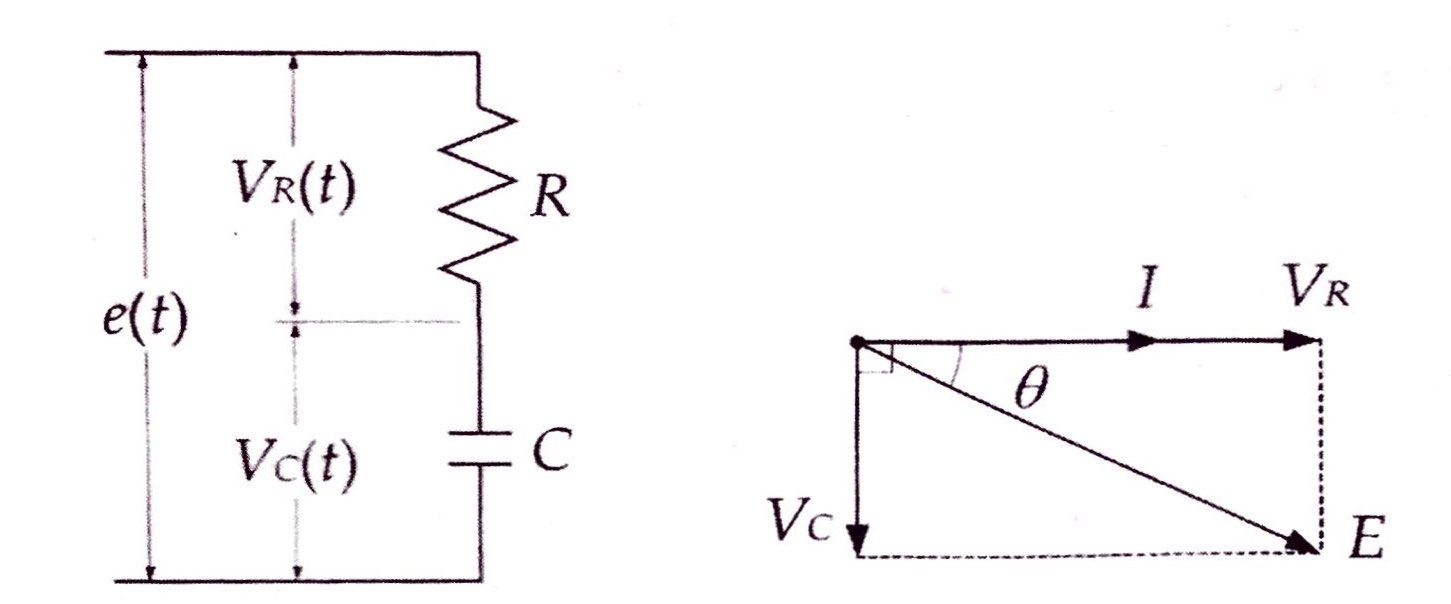
\includegraphics[bb=0 0 1451 604,height=5cm]{report3_fig3.24.jpg}
    \end{center}
    \caption{$RC$直列回路}
    \label{fig1}
\end{figure}
を得る。ただし、
\begin{eqnarray}
    Z&=&R+\frac{1}{j\omega C}=R-\frac{j}{\omega C} \label{eq9}\\
    |Z|&=&\sqrt{R^2+{\left(\frac{1}{\omega C}\right)}^2} \label{eq10}\\
    \theta&=&\tan^{-1}\left(-\frac{1}{\omega CR}\right) \label{eq11}
\end{eqnarray}
であり、$Z$を$RC$直列回路の複素インピーダンスと呼ぶ。また、
\begin{equation}
    -j=e^{-j\frac{\pi}{2}}
    \label{eq12}
\end{equation}
なので、
\begin{eqnarray}
    V_R&=&RI \label{eq13}\\
    V_C&=&\frac{1}{\omega C}I\cdot e^{-j\frac{\pi}{2}} \label{eq14}
\end{eqnarray}
であり、$E$、$I$、$V_R$、$V_C$を複素平面上でフェーザ表示(ベクトル表示)すると、
図\ref{fig1}のようになる。

$V_R$と$I$は同位相であり、$V_C$の位相は$I$より$\frac{\pi}{2}$だけ遅れている。
また、$V_R$及び$I$は$E$より$\theta$だけ位相が進んでいる。
また、$V_R$と$V_C$のベクトル和は$E$に等しい。

なお、フェーザ図(ベクトル図)から、$E$、$R$、$C$を一定として、
周波数$f$を変化させたときの位相差$\theta$が
\begin{equation}
    \theta=\tan^{-1}\left(-\frac{|V_C|}{|V_R|}\right)
    \label{eq15}
\end{equation}
で求められる。

\clearpage

\subsection{$RL$直列回路}
$RL$直列回路図\ref{fig2}の$RL$直列回路の抵抗$R$に電流$i(t)$を流した時、
抵抗$R$の両端に生じる電圧$v_R(t)$は、$RC$直列回路と同様に、
オームの法則から(\ref{eq1})式により与えられる。
一方で、インダクタンス$L$に電流$i(t)$が流れる時、
レンツの法則によってインダクタンス$L$の両端に生じる電圧$v_L(t)$は
\begin{equation}
    v_L(t)=L\frac{di(t)}{dt}
    \label{eq16}
\end{equation}
で与えられる。$RC$直列回路の場合と同様に、(\ref{eq1})式と(\ref{eq16})式から電圧$E$と電流$I$の関係式
\begin{equation}
    I=\frac{1}{Z}E=\frac{1}{|Z|}E\cdot e^{-j\theta}
    \label{eq17}
\end{equation}
を得る。ただし、
\begin{eqnarray}
    Z&=&R+j\omega L \label{eq18}\\
    |Z|&=&\sqrt{R^2+\left(\omega L\right)^2} \label{eq19}\\
    \theta&=&\tan^{-1}\left(\frac{\omega L}{R}\right) \label{eq20}
\end{eqnarray}
であり、$Z$を$RL$直列回路の複素インピーダンスと呼ぶ。また、
\begin{equation}
    v_L(t)=\sqrt{2}V_L\cdot e^{j\omega t}
    \label{eq21}
\end{equation}
とすると、
\begin{eqnarray}
    V_R&=&RI \label{eq22}\\
    V_L&=&\omega LI\cdot e^{j\frac{\pi}{2}} \label{eq23}
\end{eqnarray}
であり、$E$、$I$、$V_R$、$V_L$を複素平面上でフェーザ表示(ベクトル表示)すると、
図\ref{fig2}のようになる。

$V_R$と$I$は同位相であり、$V_L$の位相は$I$より$\frac{\pi}{2}$だけ進んでいる。
また、$V_R$および$I$は$E$より$\theta$だけ位相が遅れている。

一般のコイルは長い導線を心材に多数回巻いて作られているので、導線の抵抗成分$r$を伴う。
この抵抗$r$をコイルの内部抵抗と呼ぶ。
このため、超電導コイルをのぞいてインダクタンス$L$のみを持つコイルは存在しない。
コイルの内部抵抗$r$は、コイルを構成する導体の断面積$S$と長さ$l$と固有抵抗値$\rho$により
\begin{equation}
    r=\frac{l}{S}\times\rho
    \label{eq24}
\end{equation}
と表される。内部抵抗$r$を考慮すれば、コイルのインピーダンス$Z_L$は
\begin{equation}
    Z_L=r+j\omega L
    \label{eq25}
\end{equation}
となり、式(\ref{eq18})、(\ref{eq19})、(\ref{eq20})、(\ref{eq22})の$R$は
\begin{equation}
    R'=R+r
    \label{eq26}
\end{equation}
に置き換える必要がある。この場合、図\ref{fig2}は図\ref{fig3}のように書き換えればよい。

\clearpage

\begin{figure}[t]
    \begin{center}
        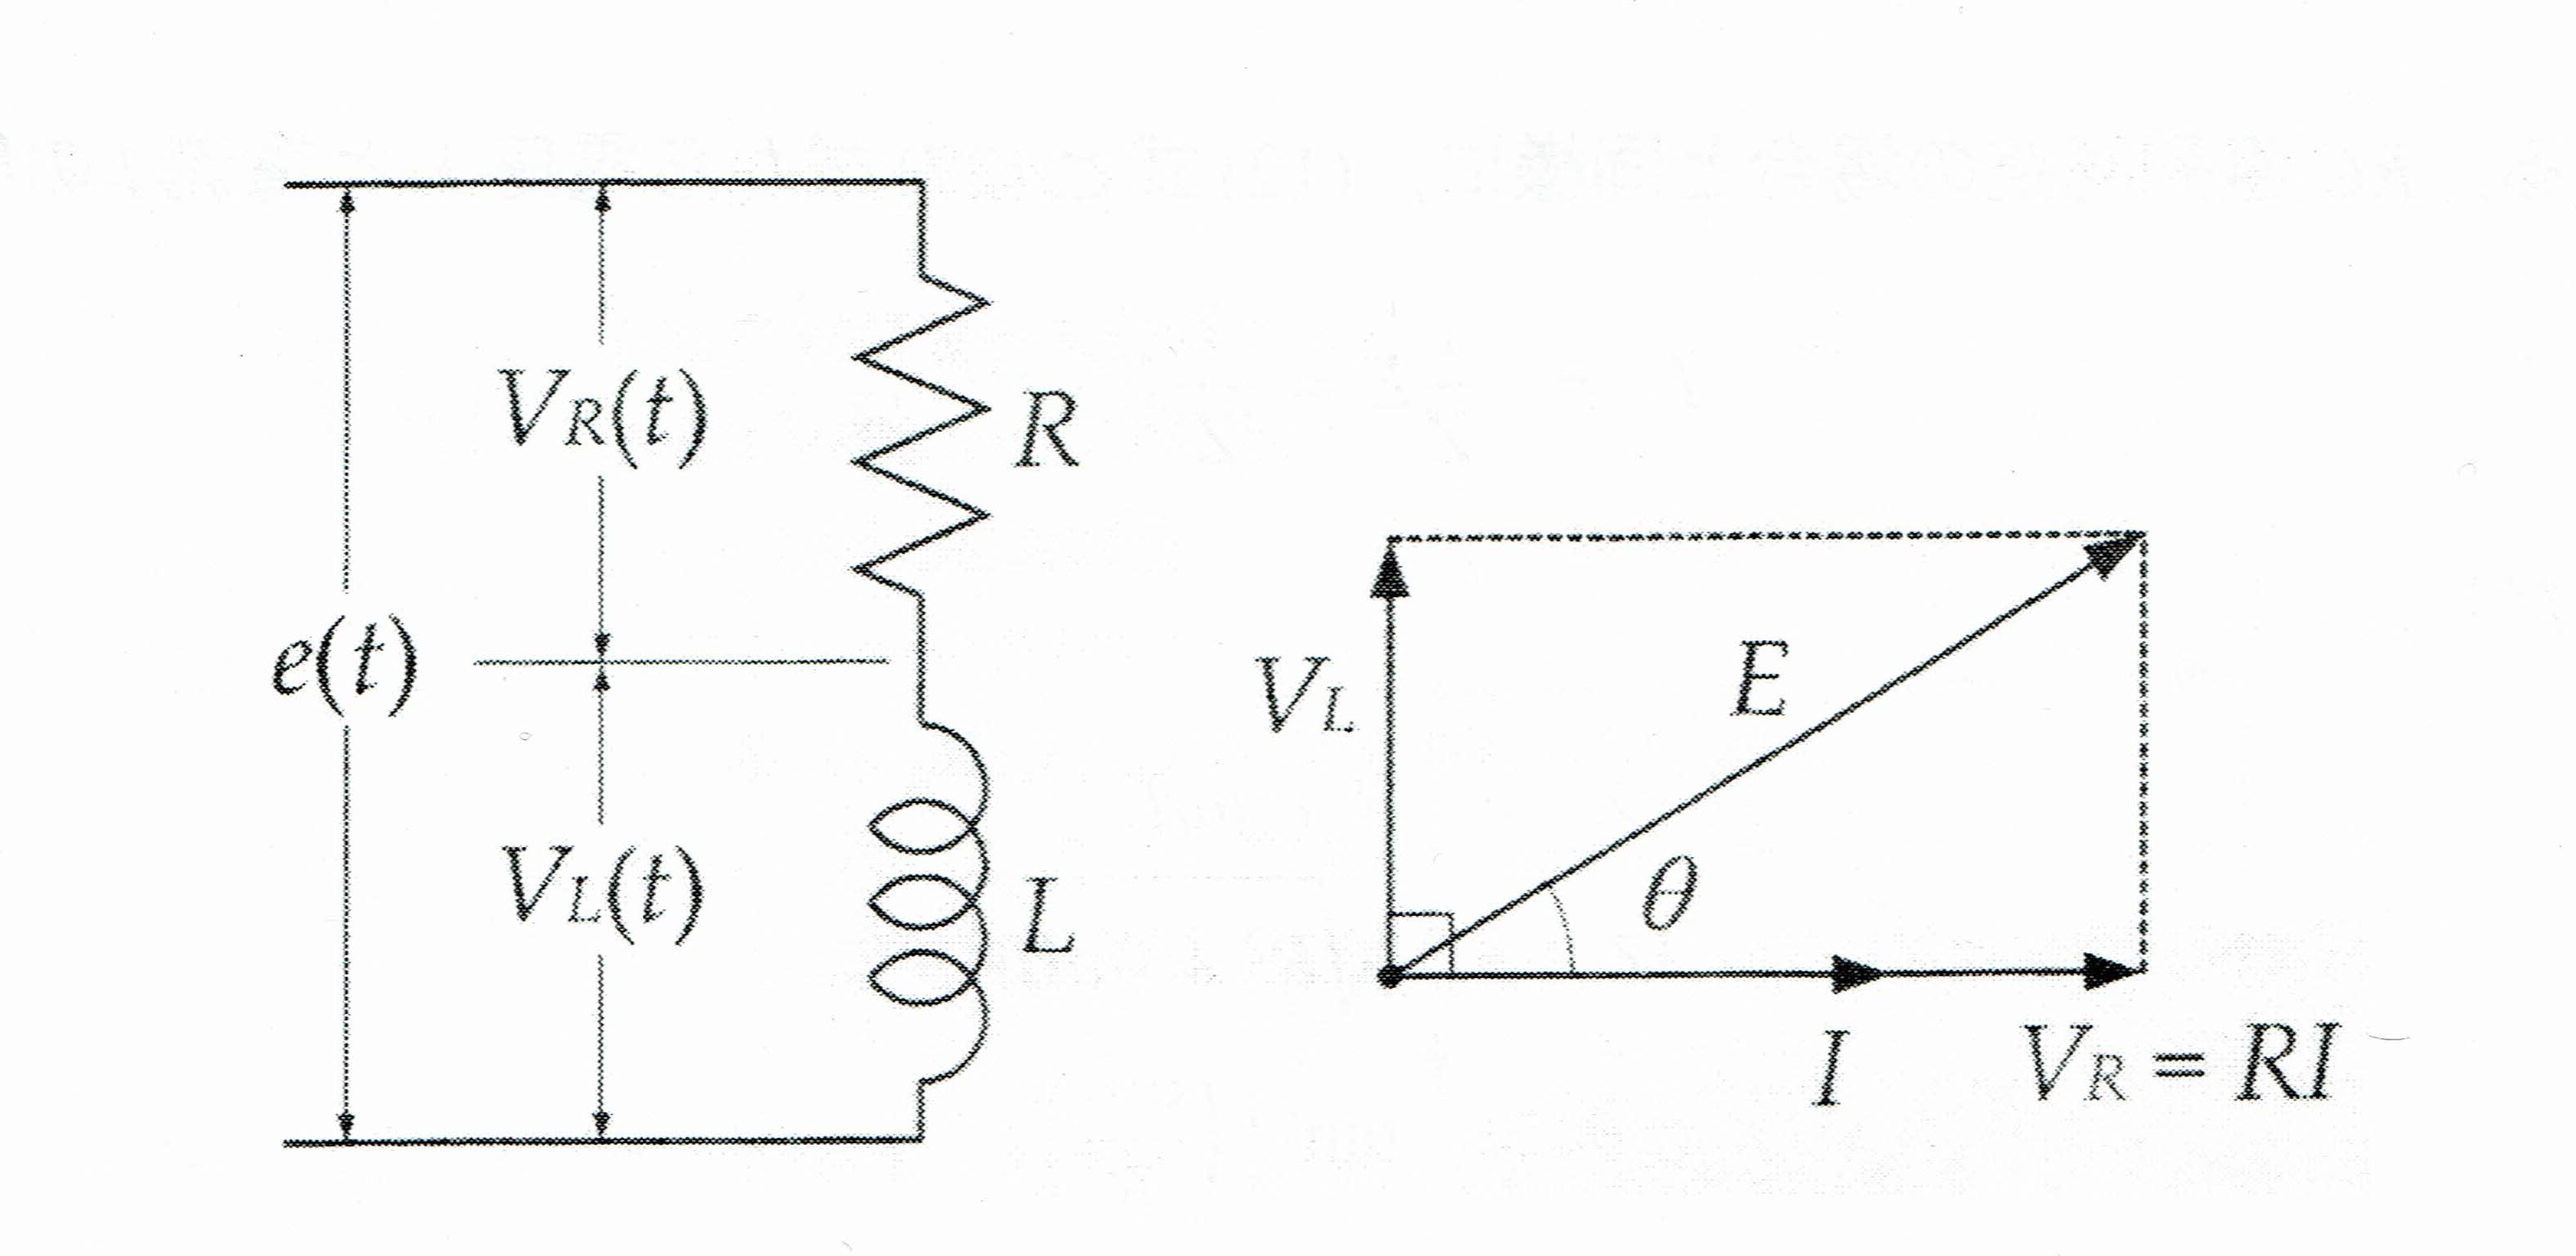
\includegraphics[bb=0 0 3151 1536,height=5cm]{report3_fig3.25.jpg}
    \end{center}
    \caption{$RL$直列回路}
    \label{fig2}
\end{figure}
\begin{figure}[t]
    \begin{center}
        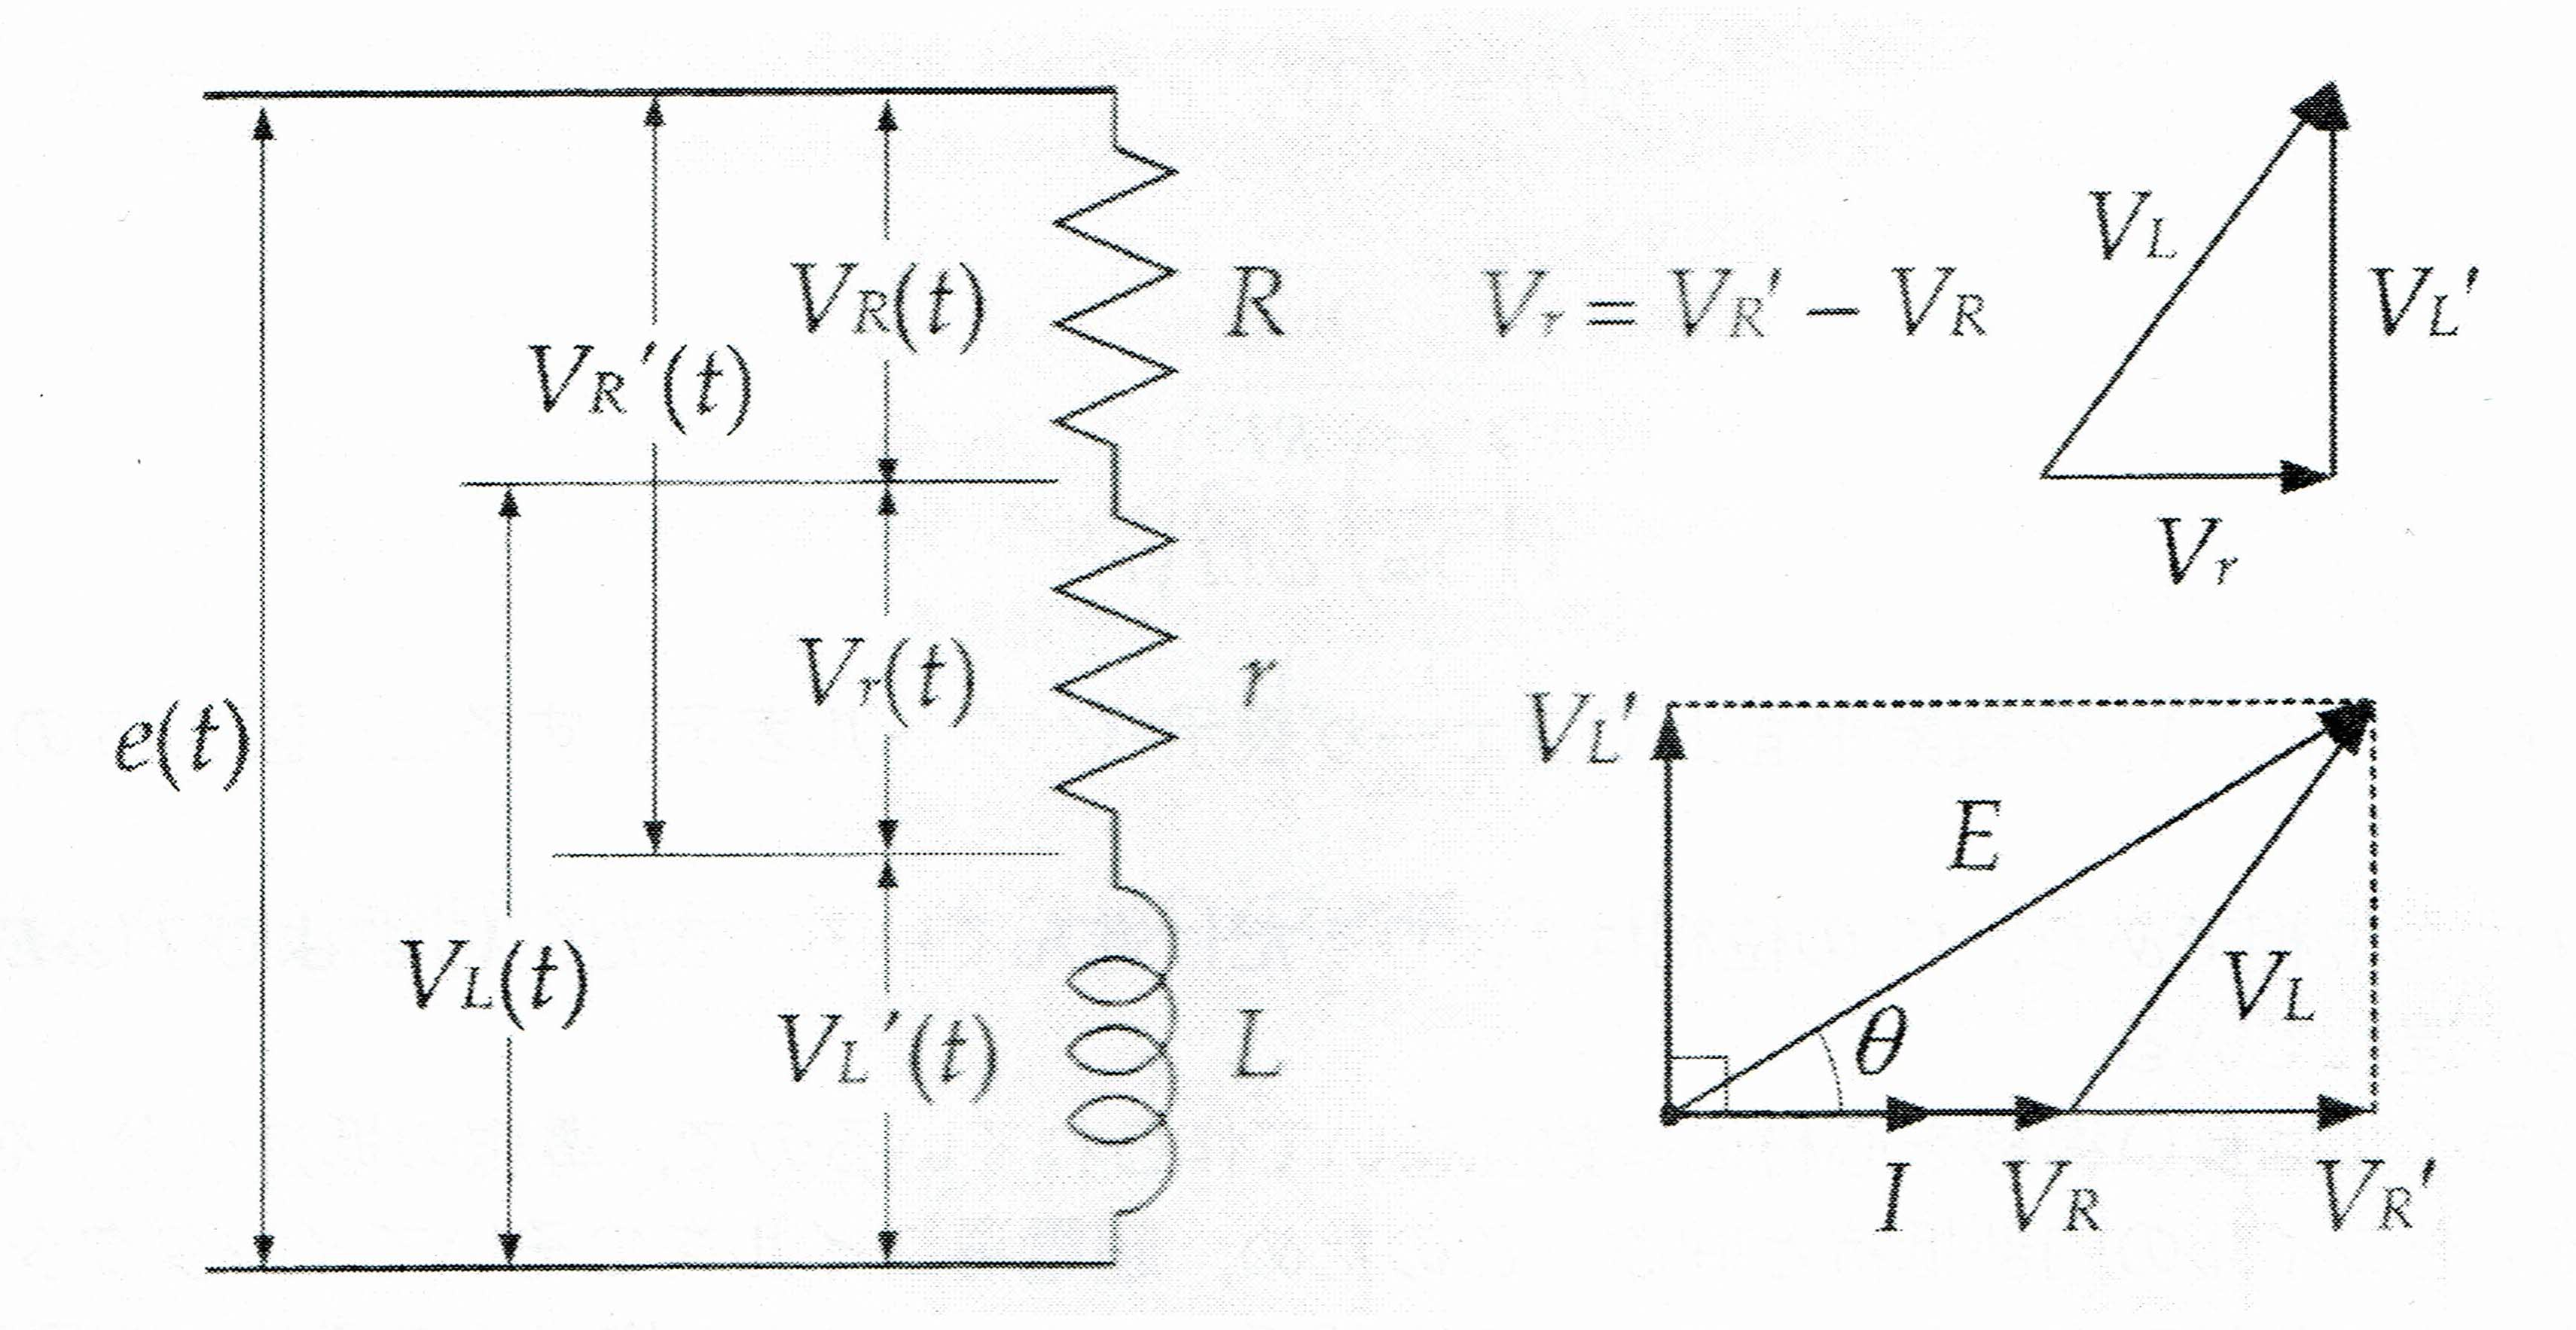
\includegraphics[bb=0 0 3420 1766,height=5cm]{report3_fig3.26.jpg}
    \end{center}
    \caption{コイルの内部抵抗$r$を考慮した$RL$直列回路}
    \label{fig3}
\end{figure}

\section{実験方法}
\subsection{$RC$直列回路}
\begin{itemize}
    \item[1)]抵抗$R$、コンデンサ$C$、発振器OSC、デジタルマルチメータDM、波形記録計RECを図\ref{fig4}のように接続する。
    \item[2)]発振器OSCの周波数$f$を設定してから電圧$E$を$1.995[{\rm V}]\sim 2.005[{\rm V}]$に調整し、
          デジタルマルチメータDMの交流電圧計で$E$、$V_R$、$V_C$を測定する。

          測定した周波数は
          $$
              f=40、60、100、200、400、600、1{\rm k}、2{\rm k}、4{\rm k}、6{\rm k}、10{\rm k}、20{\rm k}、40{\rm k}[{\rm Hz}]
          $$
          である。

          周波数毎に測定した$E$、$V_R$、$V_C$を記録するとともに、$f-V_R$、$f-V_C$の関係を両対数グラフにプロットし、
          $E'$と$\Delta E$を
          \begin{eqnarray}
              E'&=&\sqrt{{V_R}^2+{V_C}^2} \label{eq27}\\
              \Delta E&=&E-E' \label{eq28}
          \end{eqnarray}
          で計算し記録する。
    \item[3)]周波数$f=200、400、1{\rm k}[{\rm Hz}]$について、
          波形記録計RECで$E$、$V_R$、$V_C$の電圧波形を記録紙に記録する。
    \item[4)]抵抗$R[{\rm \Omega}]$とコンデンサ$C[{\rm \mu F}]$の値をLCRメータで測定し記録する。
\end{itemize}

\subsection{$RL$直列回路}
\begin{itemize}
    \item[1)]抵抗$R$、コイル$L$、発振器OSC、デジタルマルチメータDM、波形記録計RECを図\ref{fig5}のように接続する。
    \item[2)]発振器OSCの周波数$f$を設定してから電圧$E$を$1.995[{\rm V}]\sim 2.005[{\rm V}]$に調整し、
          デジタルマルチメータDMの交流電圧計で$E$、$V_R$、$V_L$を測定する。

          測定した周波数は
          $$
              f=40、60、100、200、400、600、1{\rm k}、2{\rm k}、4{\rm k}、6{\rm k}、10{\rm k}、20{\rm k}、40{\rm k}[{\rm Hz}]
          $$
          である。

          周波数毎に測定した$E$、$V_R$、$V_L$を記録するとともに、$f-V_R$、$f-V_L$の関係を両対数グラフにプロットし、
          $E'$と$\Delta E$を
          \begin{eqnarray}
              E'&=&\sqrt{{V_R}^2+{V_L}^2} \label{eq29}\\
              \Delta E&=&E-E' \label{eq30}
          \end{eqnarray}
          で計算し記録する。
    \item[3)]周波数$f=200、400、1{\rm k}[{\rm Hz}]$について、
          波形記録計RECで$E$、$V_R$、$V_L$の電圧波形を記録紙に記録する。
    \item[4)]抵抗$R[{\rm \Omega}]$とコイルのインダクタンス$L[{\rm mH}]$の値をLCRメータで測定し記録する。
\end{itemize}

\begin{figure}[t]
    \begin{minipage}{0.5\hsize}
        \begin{center}
            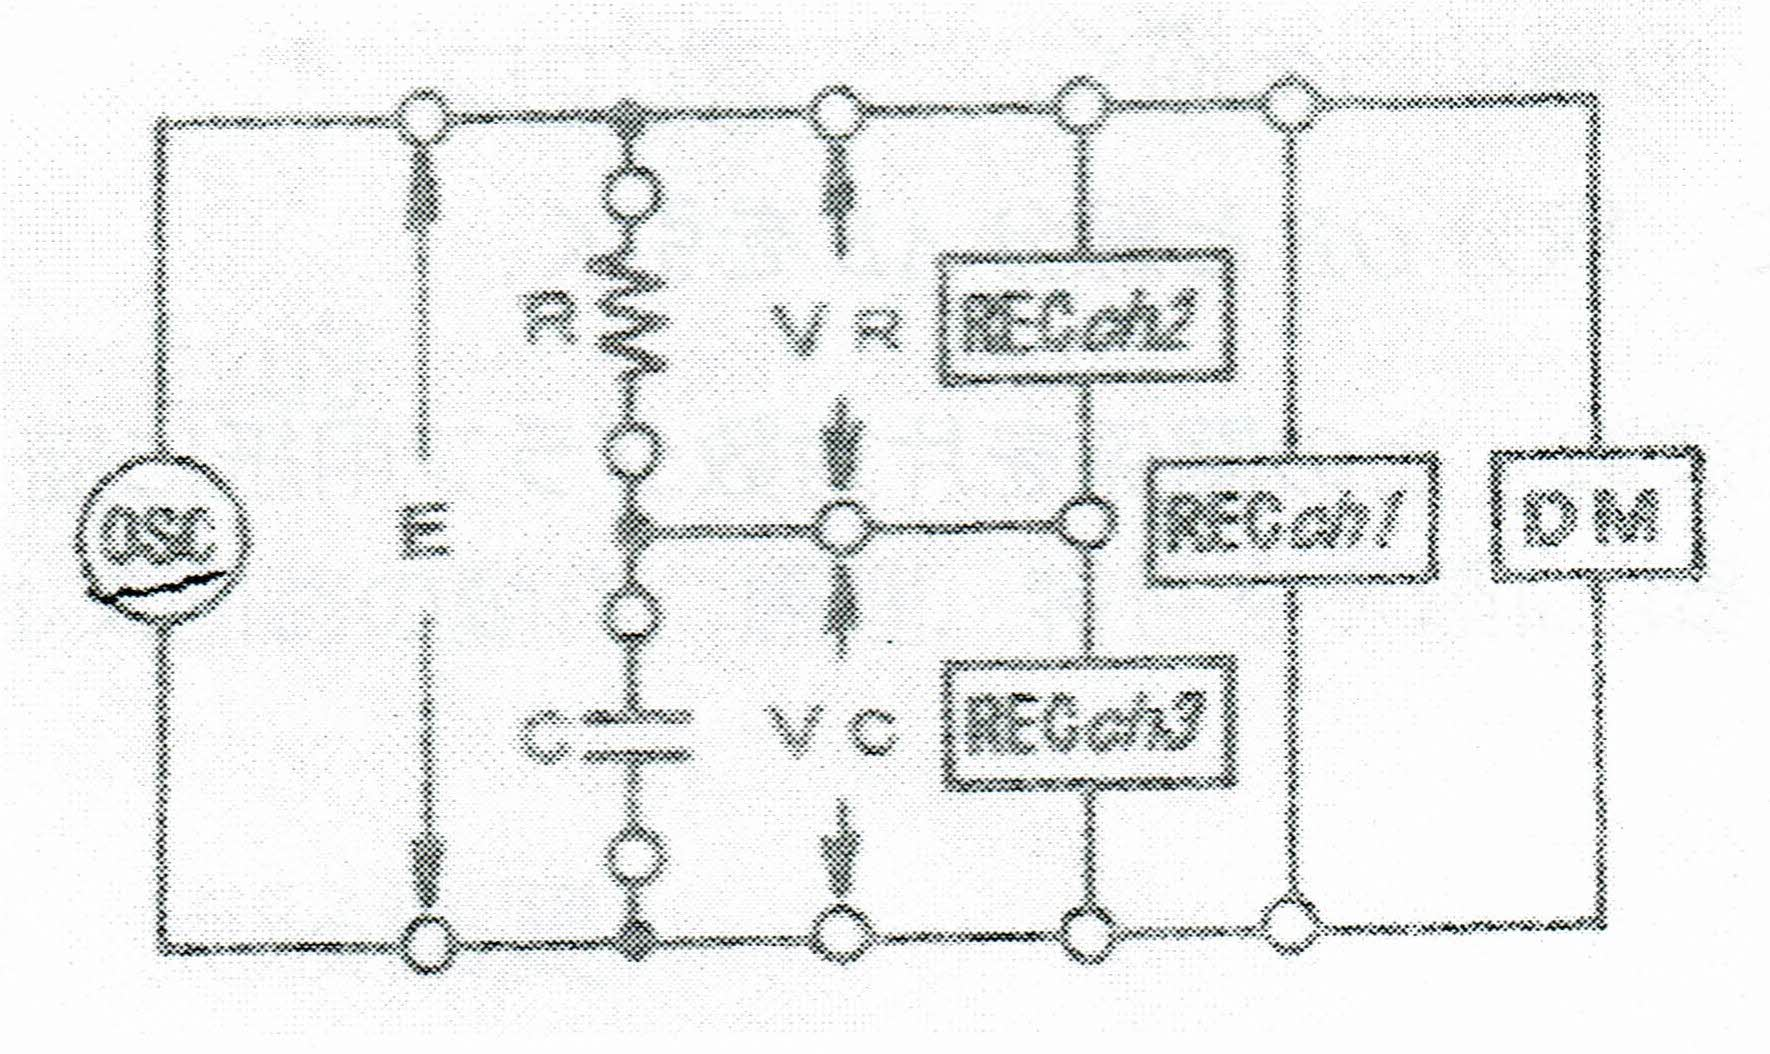
\includegraphics[bb=0 0 1770 1054,height=5cm]{report3_fig3.27.jpg}
        \end{center}
        \caption{$RC$直列回路}
        \label{fig4}
    \end{minipage}
    \begin{minipage}{0.5\hsize}
        \begin{center}
            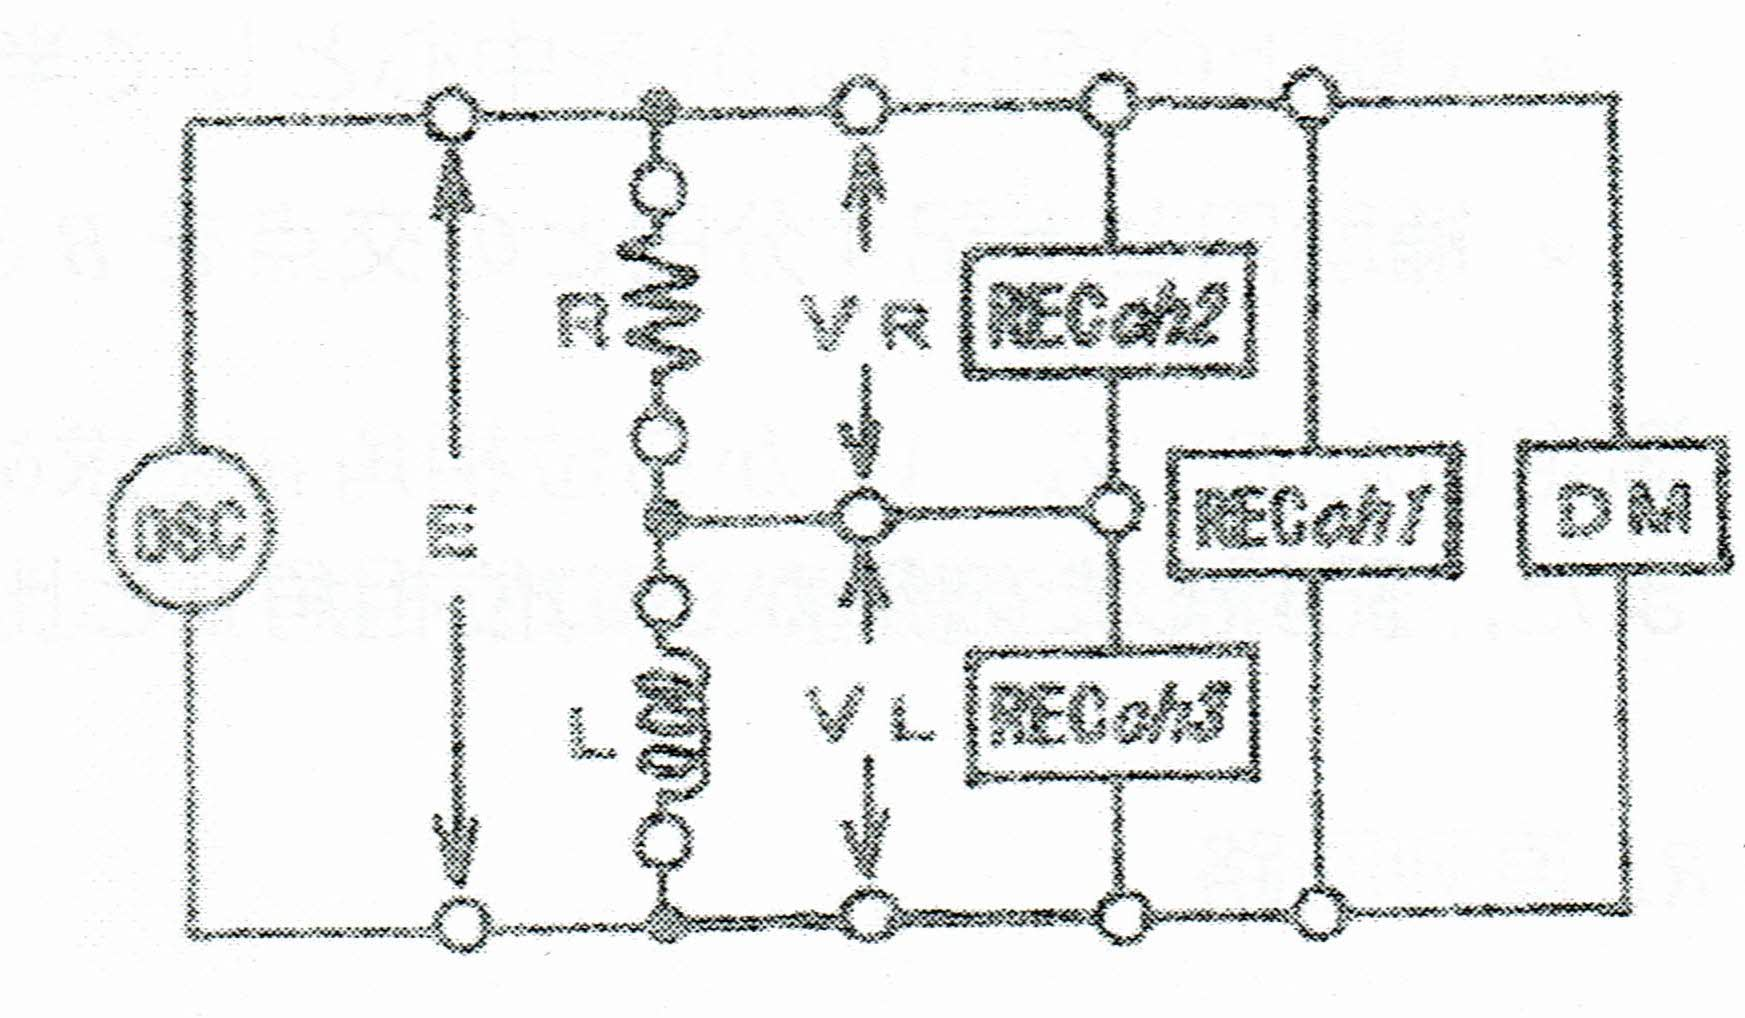
\includegraphics[bb=0 0 1745 1018,height=5cm]{report3_fig3.28.jpg}
        \end{center}
        \caption{$RL$直列回路}
        \label{fig5}
    \end{minipage}
\end{figure}

\clearpage

\section{検討・考察}
\subsection{レポート課題1}
\begin{shadebox}
    電気回路においては、電源が交流電源である場合、
    どのような回路構成でも各素子($R$、$L$、$C$)にかかる電圧(電位差)と
    それらに流れる電流には位相差が生じる。
    その要因を複素平面上の幾何学的解釈に基づいて考察せよ。
\end{shadebox}

直列回路の場合、図\ref{fig1}と図\ref{fig2}にある複素平面から分かるように、
抵抗の電圧$V_R$と電流$I$は同位相であり、
コンデンサの電圧$V_C$の位相は$I$より$\frac{\pi}{2}$だけ遅れていて、
インダクタンスの電圧$V_L$の位相は$I$より$\frac{\pi}{2}$だけ位相が進んでいる。
したがって、$RC$、$RL$、$RLC$直列回路における電圧$E$は、
それぞれ$V_R$、$V_C$、$V_L$の合成ベクトルで表せるので、
電圧と電流には位相差が生じる。
ただし、$V_C$、$V_L$が、
\begin{eqnarray}
    V_C=0、V_L=0 \label{eq31}\\
    V_C=V_L \label{eq32}
\end{eqnarray}
のどちらかを満たしているとき位相差は生じない。
また、もちろん抵抗$R$のみの回路構成の場合は、位相差が生じない。

これは、インダクタンスの電圧$V_L$が電流の変化によって生じる逆起電力によって生じることと、
コンデンサの電圧$V_C$がコンデンサにたまって形成されることが関わって位相差が生じている。

また並列回路の場合、直列回路と同様にして
図\ref{fig6}と図\ref{fig7}にある複素平面から分かるように、
抵抗の電流$I_R$と電流$E$は同位相であり、
コンデンサの電流$I_C$の位相は$E$より$\frac{\pi}{2}$だけ進んでいて、
インダクタンスの電流$I_L$の位相は$E$より$\frac{\pi}{2}$だけ位相が遅れている。
したがって、$RC$、$RL$、$RLC$並列回路における電流$I$は、
それぞれ$I_R$、$I_C$、$I_L$の合成ベクトルで表せるので、
電圧と電流には位相差が生じる。
ただし、$I_C$、$I_L$が、
\begin{eqnarray}
    I_C=0、I_L=0 \label{eq33}\\
    I_C=I_L \label{eq34}
\end{eqnarray}
のどちらかを満たしているとき位相差は生じない。
また、直列回路と同様にもちろん抵抗$R$のみの回路構成の場合は、位相差が生じない。

\clearpage

\subsection{レポート課題2}
\begin{shadebox}
    テキスト中の図3.24(レポートでは図\ref{fig1})では$R$、$C$が直列接続されているが、
    これらを並列接続したときにそれぞれの素子に流れる電流の様子を複素平面上で図示せよ。
\end{shadebox}

\begin{figure}[h]
    \begin{center}
        \begin{picture}(200,150)
            \put(190,15){$E$}
            \put(15,15){\vector(1,0){170}}

            \put(15,125){$I_C=\omega CE$}
            \put(15,15){\textcolor{red}{\vector(0,1){100}}}

            \put(110,0){$I_R=\frac{E}{R}$}
            \put(15,15){\textcolor{red}{\vector(1,0){150}}}

            \put(170,120){$I$}
            \put(15,15){\textcolor{red}{\vector(3,2){150}}}

            \put(15,15){\dashbox{10}(150,100)}

            \put(55,25){$\theta$}
            \qbezier(45,35)(50,30)(50,15)

            \put(15,15){\dashbox{10}(10,10)}
        \end{picture}
    \end{center}
    \caption{$RC$並列回路}
    \label{fig6}
\end{figure}

抵抗$R$とコンデンサ$C$が並列接続されているとき、
抵抗とコンデンサのそれぞれ両端に生じる電圧$E$は同じなので、
電圧$E$を基準にして複素平面上で図示すると図\ref{fig6}のような概形となる。

$RC$並列回路では、抵抗$R$に流れる電流$I_R$は電圧$E$と同相になり、
コンデンサ$C$に流れる電流$I_C$は電圧$E$より位相が$\frac{\pi}{2}$進む。


\subsection{レポート課題3}
\begin{shadebox}
    $R$、$L$が並列接続された場合についても上記と同様のことを行え。
\end{shadebox}

\begin{figure}[h]
    \begin{center}
        \begin{picture}(200,150)
            \put(190,115){$E$}
            \put(15,115){\vector(1,0){170}}

            \put(15,0){$I_L=\frac{E}{\omega L}$}
            \put(15,115){\textcolor{red}{\vector(0,-1){100}}}

            \put(110,125){$I_R=\frac{E}{R}$}
            \put(15,115){\textcolor{red}{\vector(1,0){150}}}

            \put(170,10){$I$}
            \put(15,115){\textcolor{red}{\vector(3,-2){150}}}

            \put(15,15){\dashbox{10}(150,100)}

            \put(55,97){$\theta$}
            \qbezier(50,115)(55,105)(45,95)

            \put(15,105){\dashbox{10}(10,10)}
        \end{picture}
    \end{center}
    \caption{$RL$並列回路}
    \label{fig7}
\end{figure}

抵抗$R$とインダクタンス$L$が並列接続されているとき、
抵抗とインダクタンスのそれぞれ両端に生じる電圧$E$は同じなので、
電圧$E$を基準にして複素平面上で図示すると図\ref{fig7}のような概形となる。

$RL$並列回路では、抵抗$R$に流れる電流$I_R$は電圧$E$と同相になり、
インダクタンス$L$に流れる電流$I_L$は電圧$E$より位相が$\frac{\pi}{2}$遅れている。

\clearpage

\section{結論}
抵抗($R$)、コンデンサ($C$)、インダクタンス($L$)からなる回路に、
正弦的に振動する電圧を加えた時に起きる現象について、
実験を行うことはできなかったが、
$RC$直列回路や$RL$直列回路の複素平面などを用いて幾何学的に理解することができた。

% 参考文献
\begin{thebibliography}{99}
    \label{sannkoubunnkenn_chapter}
    \bibitem[1]{rikadai}東京理科大学工学部情報工学科「情報工学実験1 2020年度」
    (2020/4/6)

    \bibitem[2]{rc_circuit}$RC$並列回路の概要

    \url{https://hegtel.com/rc-heiretsu.html}

    最終閲覧日:2020/6/9

    \bibitem[3]{rl_circuit}$RL$並列回路の概要

    \url{https://hegtel.com/rl-heiretsu.html}

    最終閲覧日:2020/6/9

    \bibitem[4]{zikken}$RLC$直列回路 - Java実験室

    \url{https://javalab.org/ja/rlc_serial_circuit_ja/}

    最終閲覧日:2020/6/9

\end{thebibliography}

\clearpage
\appendix
%%%%%%%%%%%%%%%%%%%%%%%%%%%%%%%%%%%%%%%%%%%%%%%%%%%%%%%
\end{document}
